\begin{frame}{Πειραματική διαδικασία: διάταξη}

  \begin{itemize}
    \item Πέντε προσομοιωμένα περιβάλλοντα / Ένα πραγματικό
    \item Προσομοιωμένα:
      \begin{itemize}
        \item 38 δοκιμαστικές στάσεις
        \item 100 επαναλήψεις ανά στάση
        \item LIDAR: $\sigma_R = \{0.01, 0.02, 0.05\}$ cm, $r_{\max} = 10.0$ m
      \end{itemize}
    \item CSAL AUTh:
      \begin{itemize}
        \item 11 δοκιμαστικές στάσεις
        \item 5 επαναλήψεις ανά στάση
        \item LIDAR: YDLIDAR TG30, $r_{\max} = 30.0$ m \\

              \noindent\makebox[0.3\linewidth][c]{%o
              \begin{minipage}{0.3\linewidth}
                \begin{figure}
                  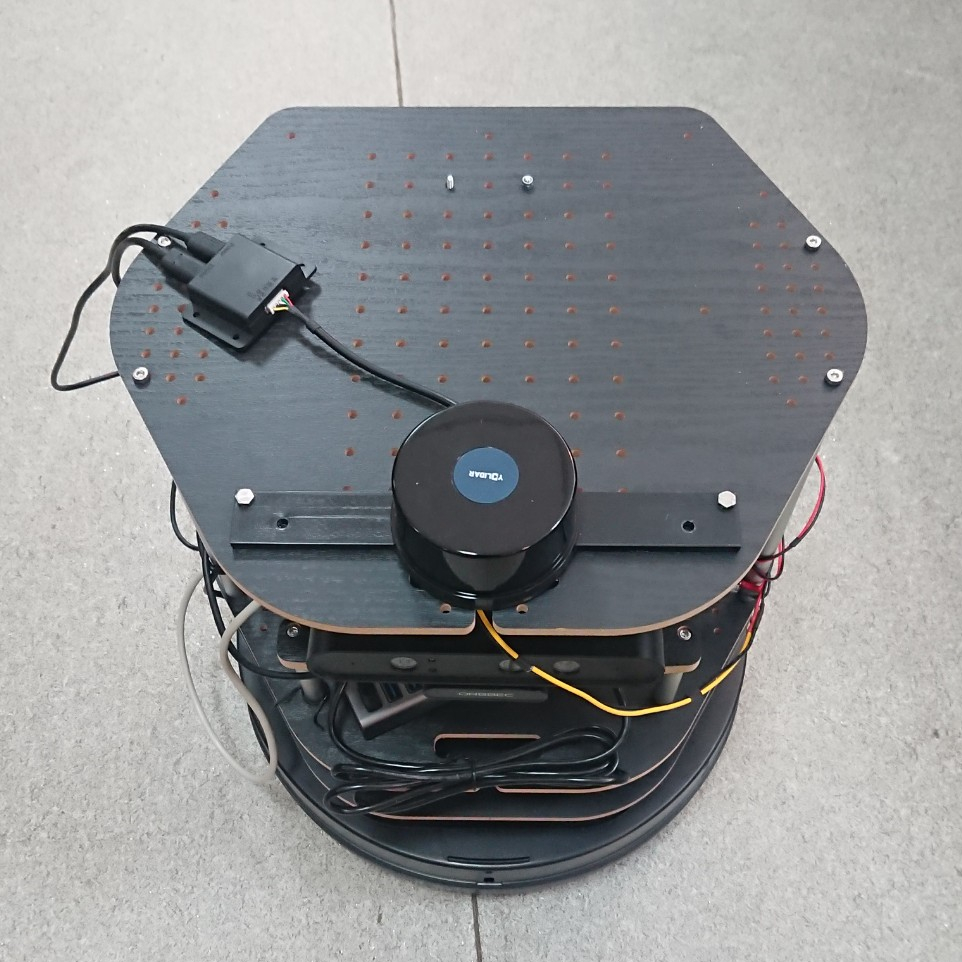
\includegraphics[scale=0.09]{./figures/slides/ch5/tb_yd.jpg}
                \end{figure}
              \end{minipage}
              }
              \hfill
              \noindent\makebox[0.6\linewidth][c]{%
              \scriptsize
              \begin{minipage}{0.6\linewidth}
                \begin{table}[h]\centering \vspace{0.5cm}
                        \begin{tabular}{rc}
                          Απόσταση $d$ [mm]    & Μέσο σφάλμα [mm]   \\ \toprule
                          $50$-$5000$          & $\leq \pm 60$      \\
                          $5000$-$20000$       & $\leq \pm 40$      \\
                          $20000$-$30000$      & $\leq \pm 100$     \\ \bottomrule
                        \end{tabular}
                        \caption{Μέσο σφάλμα μέτρησης αισθητήρα ανά επιστρεφόμενη τιμή απόστασης. Πηγή: datasheet κατασκευαστή}
                \end{table}
              \end{minipage}
    }
    \end{itemize}
  \end{itemize}


\note{\footnotesize
Για να δοκιμαστεί εάν το πρόβλημα της ανεύρεσης της στάσης ενός ρομπότ που
είναι εξοπλισμένο με έναν πανοραμικό αισθητήρα lidar είναι επιλύσιμο μέσω sm2
χωρίς αντιστοιχίσεις: δοκιμάζουμε το σύστημα επίλυσης σε πέντε προσομοιωμένα
περιβάλλοντα και ένα πραγματικό, για συνολικά 49 στάσεις, οι οποίες
δημιουργήθηκαν είτε τυχαία είτε έτσι ώστε να δοκιμάσουν την επίδοση των μεθόδων
sm2 που θα δοκιμαστούν σε αυτό το πρόβλημα. Τα πειράματα στα προσομοιωμένα
περιβάλλοντα επαναλήφθηκαν για 100 φορές ανά στάση, και στο πραγματικό
περιβάλλον για 5 φορές ανά στάση.  Στα προσομοιωμένα περιβάλλοντα
χρησιμοποιούμε έναν πανοραμικό αισθητήρα lidar μεγίστου βεληνεκούς δέκα μέτρων
με θόρυβο μέτρησης κανονικά κατανεμημένο, με τιμές τυπικής απόκλισης 1,2,και 5
εκατοστά, ενώ στα πραγματικά πειράματα χρησιμοποιούμε έναν αισθητήρα YDLIDAR
μέγιστου βεληνεκούς τριάντα μέτρων με κατανομή θορύβου μέτρησης που φαίνεται σε
αυτόν τον πίνακα.}

\end{frame}
